\documentclass[11pt]{article}

\usepackage[margin=1in]{geometry}
\usepackage{graphicx}
\usepackage{booktabs}
\usepackage{longtable}
\usepackage{array}
\usepackage{enumitem}
\usepackage{hyperref}
\usepackage{url}
\usepackage{xcolor}
\usepackage{float}
\usepackage[T1]{fontenc}
\usepackage[utf8]{inputenc}
\usepackage{lmodern}

\graphicspath{{../../evals/figures/}}

\hypersetup{
  colorlinks=true,
  linkcolor=blue,
  urlcolor=blue
}

\newcolumntype{L}[1]{>{\raggedright\arraybackslash}p{#1}}
\setlist[itemize]{leftmargin=*}
\setlist[enumerate]{leftmargin=*}

\begin{document}

\begin{titlepage}
\centering
\vspace*{1.5cm}
{\Large \textbf{CISC 856 - Reinforcement Learning}}\\[2.5cm]
{\Large \textbf{Final Project Report}}\\[2.5cm]
{\LARGE Benchmarking DQN, PPO, and DiscreteSAC on Atari 2600 Games}\\[2.5cm]
{\large \textbf{Group 4:}}\\[0.8cm]
{\large Elsayed Elmandoh}\\[0.25cm]
{\large Mohamed Hasan}\\[0.25cm]
{\large Mohamed Zidan}\\[0.25cm]
{\large Mostafa Elofy}
\vfill
\end{titlepage}

\section*{1 - Introduction}

Atari 2600 environments are a standard testbed for deep reinforcement learning because they combine high-dimensional visual observations, delayed rewards, partial observability, action repeat, stochastic initial states, and game-specific control patterns. This project uses Atari as a compact but meaningful benchmark for comparing value-based, policy-gradient, and maximum-entropy reinforcement learning methods under a shared experimental pipeline.

The project focuses on three games: Pong, Breakout, and Space Invaders. These games were selected because they stress different learning behaviors. Pong requires fast paddle tracking and opponent reaction. Breakout requires paddle control, ball recovery, and sustained rallies. Space Invaders requires shooting, lateral positioning, and survival under incoming enemy fire. These differences make the benchmark more informative than testing a single Atari game.

The algorithms are DQN, PPO, and DiscreteSAC. DQN and PPO are implemented using Stable Baselines3 because they are mature reference baselines. SAC is more complicated: the standard Stable Baselines3 SAC implementation is for continuous action spaces, while Atari uses discrete action spaces. Therefore, this project uses a custom \texttt{DiscreteSAC} implementation with a categorical policy over the Atari action set.

The goal is not only to produce final reward numbers, but to build an end-to-end benchmark system that can be inspected and reproduced. The repository includes configuration files, source code, checkpoints, CSV result files, manifests, diagnostics, TensorBoard logs, input samples, and MP4 playback videos. This follows the project guidance in \path{docs/project-definition/making-a-rewarding-rl-project.md}: use existing tools where appropriate, define the RL problem rigorously, conduct comprehensive experiments, and discuss failures honestly.

The final evidence emphasized in this report is stored in one profile-scoped benchmark location. The completed final comparison now uses the same profile, games, and seeds for all three algorithms.

\begin{longtable}{L{0.18\textwidth} L{0.37\textwidth} L{0.37\textwidth}}
\toprule
Algorithm & Final playback folder & Final checkpoint/results folder \\
\midrule
\endhead
DQN & \path{artifacts/evaluation/playback/1m_5seeds/} & \path{evals/checkpoints/1m_5seeds/} \\
PPO & \path{artifacts/evaluation/playback/1m_5seeds/} & \path{evals/checkpoints/1m_5seeds/} \\
DiscreteSAC & \path{artifacts/evaluation/playback/1m_5seeds/} & \path{evals/checkpoints/1m_5seeds/} \\
\bottomrule
\end{longtable}

Older and shorter profiles are still discussed because they explain how the benchmark evolved, but the final comparison highlights the \texttt{1m\_5seeds} folders above.

\section*{2 - Problem Formulation}

\subsection*{Environment Set}

The benchmark uses Gymnasium with the Arcade Learning Environment. Environment IDs are resolved through \path{configs/envs.json} and \path{src/utils/data_acquisition.py}.

\begin{longtable}{L{0.22\textwidth} L{0.25\textwidth} L{0.43\textwidth}}
\toprule
Game & Resolved environment & Main challenge \\
\midrule
\endhead
Pong & \texttt{ALE/Pong-v5} & Track ball position and move paddle reactively \\
Breakout & \texttt{ALE/Breakout-v5} & Keep ball alive, return shots, break bricks \\
Space Invaders & \texttt{ALE/SpaceInvaders-v5} & Shoot enemies while moving and avoiding bullets \\
\bottomrule
\end{longtable}

\subsection*{State Space}

At each time step, the raw Atari state is an RGB frame:

\begin{verbatim}
s_raw in {0, ..., 255}^(210 x 160 x 3)
\end{verbatim}

The benchmark does not feed raw RGB frames directly to the models. All algorithms share the same preprocessing pipeline from \path{configs/preprocessing.json}:

\begin{enumerate}
\item no-op reset with \texttt{noop\_max = 30};
\item frame skip/action repeat with \texttt{frame\_skip = 4};
\item grayscale conversion;
\item resize to \texttt{84 x 84};
\item stack the four most recent processed frames.
\end{enumerate}

The final model input is:

\begin{verbatim}
s in {0, ..., 255}^(4 x 84 x 84)
\end{verbatim}

The layout is channel-first \texttt{(C, H, W)}, dtype is \texttt{uint8}, and model code normalizes observations to \texttt{[0, 1]} before neural-network computation. The input contract is checked before training: shape, dtype, range, layout, contiguity, batch dimension, and prediction compatibility are validated.

\subsection*{Action Space}

Each Atari environment has a discrete action space:

\begin{verbatim}
a in {0, 1, ..., n - 1}
\end{verbatim}

Breakout uses four actions in this setup. Pong and Space Invaders use six actions, generally corresponding to combinations such as \texttt{NOOP}, \texttt{FIRE}, \texttt{RIGHT}, \texttt{LEFT}, \texttt{RIGHTFIRE}, and \texttt{LEFTFIRE}. Playback now records action meanings when available, because action counts are easier to interpret when the report can connect action IDs to game controls.

\subsection*{Reward Function}

The environment reward is the score delta returned by ALE:

\begin{verbatim}
r_t = R(s_t, a_t, s_{t+1})
\end{verbatim}

Training uses reward clipping where configured:

\begin{verbatim}
clipped_reward = clip(r_t, -1, 1)
\end{verbatim}

Evaluation reports accumulated game reward across full episodes. The benchmark records mean reward, standard deviation, minimum, maximum, wall-clock training time, reward per hour, checkpoint paths, diagnostics paths, playback paths, playback step counts, and playback action counts.

No custom shaping reward was added for aiming, dodging, or paddle tracking. For example, Space Invaders does not directly reward dodging bullets; survival is learned indirectly from longer episodes and continued scoring opportunities. This is important when interpreting weak Space Invaders policies that learn to shoot but do not dodge well.

\section*{3 - Solution Overview}

\subsection*{Repository Architecture}

The project is organized as a reproducible benchmark pipeline.

\begin{longtable}{L{0.23\textwidth} L{0.67\textwidth}}
\toprule
Path & Purpose \\
\midrule
\endhead
\path{app.py} & Main benchmark runner: profiles, locks, training, evaluation, playback, CSV/manifest writing \\
\path{configs/} & Algorithms, environments, preprocessing, profiles, model contracts, defaults \\
\path{src/config/} & Settings, logging, config loading, config hashing \\
\path{src/utils/} & Atari environment construction, wrappers, seed/device helpers \\
\path{src/models/} & DQN, PPO, DiscreteSAC, SB3 bridge, training/evaluation harness \\
\path{src/evaluation/} & Input validation, metadata, metrics, reporting helpers \\
\path{src/inference/} & Playback regeneration from saved checkpoints \\
\path{evals/} & Checkpoints, result CSVs, manifests, diagnostics, figures \\
\path{artifacts/} & Input frame samples and playback videos \\
\path{logs/} & TensorBoard event files and process logs \\
\path{docs/} & Proposal, project definition, reference guide, final report \\
\bottomrule
\end{longtable}

\subsection*{Experiment Profiles}

The benchmark is profile-based. A profile controls timesteps, seeds, evaluation episodes, and checkpoint frequency. Important profiles include:

\begin{longtable}{L{0.35\textwidth} L{0.55\textwidth}}
\toprule
Profile & Purpose \\
\midrule
\endhead
\texttt{100k\_1seed} & Early pilot across all algorithms and games \\
\texttt{200k\_1seed} & Tuned pilot after initial stability issues \\
\texttt{300k\_1seed\_ppo\_sac\_improved} & Quick PPO and DiscreteSAC comparison, DQN excluded \\
\texttt{1m\_5seeds} & Final multi-seed benchmark folder for DQN, PPO, and DiscreteSAC \\
\texttt{1m\_1seed\_ppo\_diagnostic} & PPO-only diagnostic run \\
\texttt{1m\_1seed\_StaDiscSac\_diagnostic} & Stable DiscreteSAC diagnostic run \\
\bottomrule
\end{longtable}

Outputs are profile-scoped:

\begin{verbatim}
evals/checkpoints/<profile>/
  <profile>_results_<timestamp>.csv
  <profile>_manifest_<timestamp>.json
  <game>/<algo>/seed_<seed>/
    final_model.zip       # DQN/PPO
    final_model.pt        # DiscreteSAC
    *_steps.zip or *.pt
    ppo_diagnostics.csv
    discrete_sac_diagnostics.csv

artifacts/evaluation/playback/<profile>/
  <game>/<algo>/*.mp4
\end{verbatim}

\subsection*{Algorithms}

\subsubsection*{DQN}

DQN is implemented with Stable Baselines3 using \texttt{CnnPolicy}. It is the most stable baseline in this project and should mostly be treated as the reference value-learning agent. It uses a replay buffer, target network updates, epsilon-greedy exploration, and one environment.

The final DQN evidence is:

\begin{itemize}
\item playback: \path{artifacts/evaluation/playback/1m_5seeds/};
\item checkpoints/results: \path{evals/checkpoints/1m_5seeds/}.
\end{itemize}

\subsubsection*{PPO}

PPO is implemented with Stable Baselines3 using \texttt{CnnPolicy} and vectorized environments. It uses clipped policy optimization, generalized advantage estimation, entropy regularization, and eight environments. PPO was given a dedicated diagnostic profile because the earlier 300k playback looked collapsed: Pong repeated one action, Breakout showed weak short-episode paddle behavior, and Space Invaders repeated one action.

The PPO diagnostic profile added:

\begin{itemize}
\item PPO-specific diagnostics through \texttt{ppo\_diagnostics.csv};
\item result CSV playback metadata;
\item profile-specific checkpoint and playback folders.
\end{itemize}

The final PPO evidence is:

\begin{itemize}
\item playback: \path{artifacts/evaluation/playback/1m_5seeds/};
\item checkpoints/results: \path{evals/checkpoints/1m_5seeds/}.
\end{itemize}

\subsubsection*{DiscreteSAC}

DiscreteSAC is custom because standard SB3 SAC is continuous-action. The project uses a categorical policy for Atari actions, twin Q networks, target Q networks, replay buffer storage, entropy temperature tuning, and diagnostics.

The DiscreteSAC implementation evolved significantly during the project. Earlier versions were fragile on Atari. Diagnostic work showed two separate issues:

\begin{enumerate}
\item the training algorithm needed more stable hyperparameters;
\item deterministic playback could make a non-deterministic policy look completely collapsed.
\end{enumerate}

The final DiscreteSAC evidence is:

\begin{itemize}
\item playback: \path{artifacts/evaluation/playback/1m_5seeds/};
\item checkpoints/results: \path{evals/checkpoints/1m_5seeds/}.
\end{itemize}

\subsection*{Problems Found And Solutions Implemented}

The project improved through several debugging cycles. The main problems and fixes are summarized below.

\begin{longtable}{L{0.29\textwidth} L{0.29\textwidth} L{0.32\textwidth}}
\toprule
Problem & Evidence & Solution \\
\midrule
\endhead
Need to prevent overlapping runs in the same profile & Long runs could accidentally reuse the same output folder & Added profile locking in \path{app.py} \\
Need to run only selected algorithms & Diagnostics required PPO-only and DiscreteSAC-only runs & Added \texttt{--algo} support with multiple algorithm names \\
Need visual inspection, not only reward tables & Playback revealed behavior collapse that scores alone hid & Added MP4 playback recording per model/game/seed \\
Playback should match evaluation environment & Training wrappers and eval wrappers differed & Playback now uses eval env overrides \\
Results needed provenance & Hard to connect CSV rows to checkpoints/videos & CSV rows now include playback info and diagnostics path \\
PPO 300k playback looked collapsed & Repeated one action in Pong/Space Invaders & Added \texttt{1m\_1seed\_ppo\_diagnostic} and \texttt{ppo\_diagnostics.csv} \\
DiscreteSAC used continuous-SAC assumptions originally avoided & Atari actions are discrete & Kept custom \texttt{DiscreteSAC}, not SB3 continuous SAC \\
DiscreteSAC gradients/Q-values could become unstable & Early Space Invaders collapse and weak behavior & Added finite-gradient guards, clipping, action logging, diagnostics \\
Earlier DiscreteSAC deterministic playback repeated one action & Pong paddle did not move usefully; Space Invaders only fired & DiscreteSAC eval/playback now supports stochastic policy sampling \\
Breakout playback could stall after ball passed paddle & Video kept recording but ball was not served again & Added post-life FIRE wrapper for full-game eval/playback \\
Need easier playback regeneration & Multiline PowerShell commands were inconvenient & Added \texttt{python -m src.inference.record\_playback <profile> <env>} \\
DiscreteSAC still underperformed reference Atari SAC recipes & Pong/Space Invaders policies remained weak & Updated recipe toward reference Atari SAC: higher entropy target, min-Q backup, delayed updates, larger batch, target refresh cadence \\
\bottomrule
\end{longtable}

\section*{4 - Results}

This section reports all major benchmark evidence, with the final quantitative comparison taken from the completed \texttt{1m\_5seeds} profile for every algorithm.

\subsection*{Final Evidence Folders}

\begin{longtable}{L{0.16\textwidth} L{0.23\textwidth} L{0.27\textwidth} L{0.27\textwidth}}
\toprule
Algorithm & Final profile & Playback evidence & Checkpoint/result evidence \\
\midrule
\endhead
DQN & \texttt{1m\_5seeds} & \path{artifacts/evaluation/playback/1m_5seeds/} & \path{evals/checkpoints/1m_5seeds/} \\
PPO & \texttt{1m\_5seeds} & \path{artifacts/evaluation/playback/1m_5seeds/} & \path{evals/checkpoints/1m_5seeds/} \\
DiscreteSAC & \texttt{1m\_5seeds} & \path{artifacts/evaluation/playback/1m_5seeds/} & \path{evals/checkpoints/1m_5seeds/} \\
\bottomrule
\end{longtable}

The final benchmark contains 45 completed runs: three algorithms, three games, and five seeds per condition (\texttt{0}, \texttt{1}, \texttt{2}, \texttt{3}, and \texttt{4}). The repository also contains one final model and one playback MP4 for each run.

\subsection*{Evaluation Figures}

The generated figures are stored in \path{evals/figures/}. They summarize the benchmark from complementary views: mean reward, best observed reward, reward normalized by wall-clock time, and training time.

\begin{figure}[H]
\centering
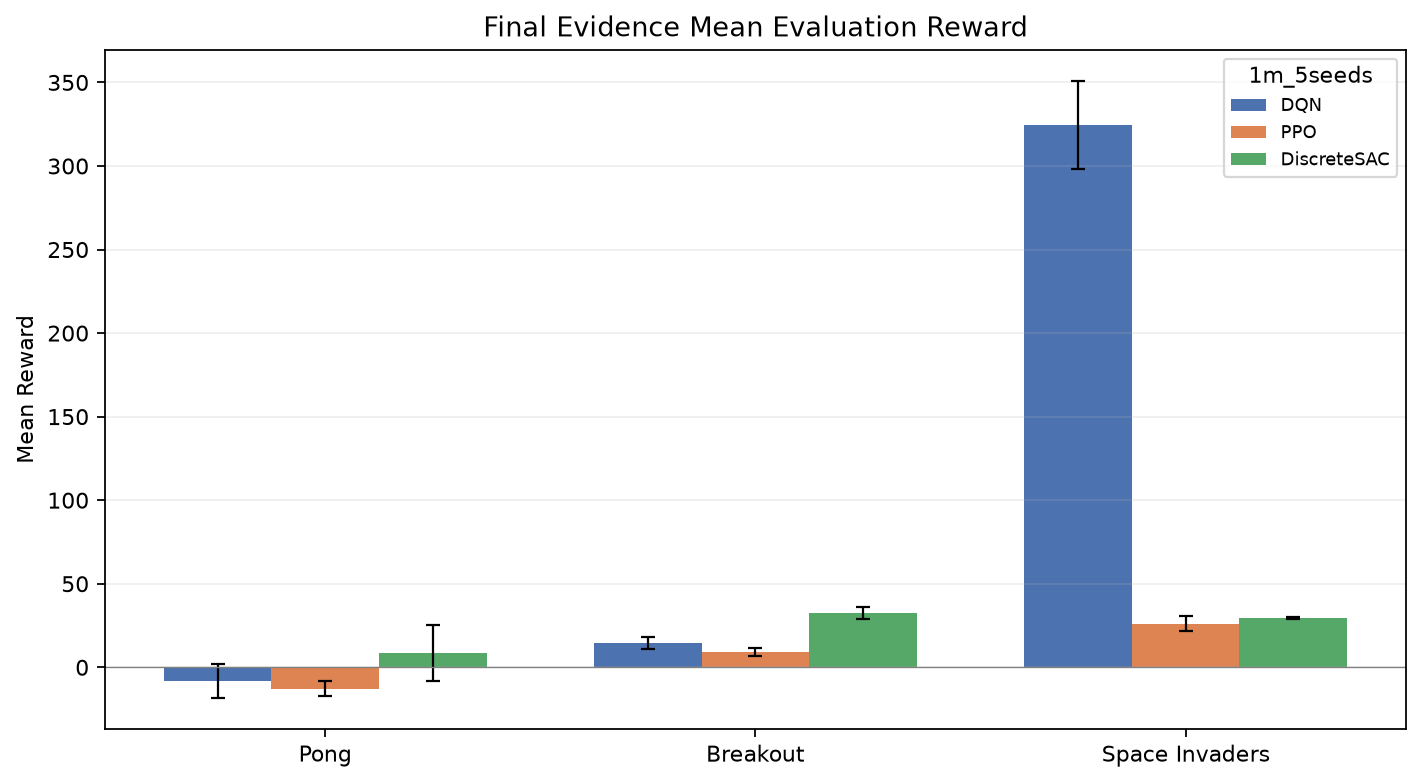
\includegraphics[width=0.95\linewidth]{mean_reward.png}
\caption{Mean reward. This plot compares average evaluation reward across benchmark conditions. It is the main quantitative view for judging final policy performance.}
\end{figure}

\begin{figure}[H]
\centering
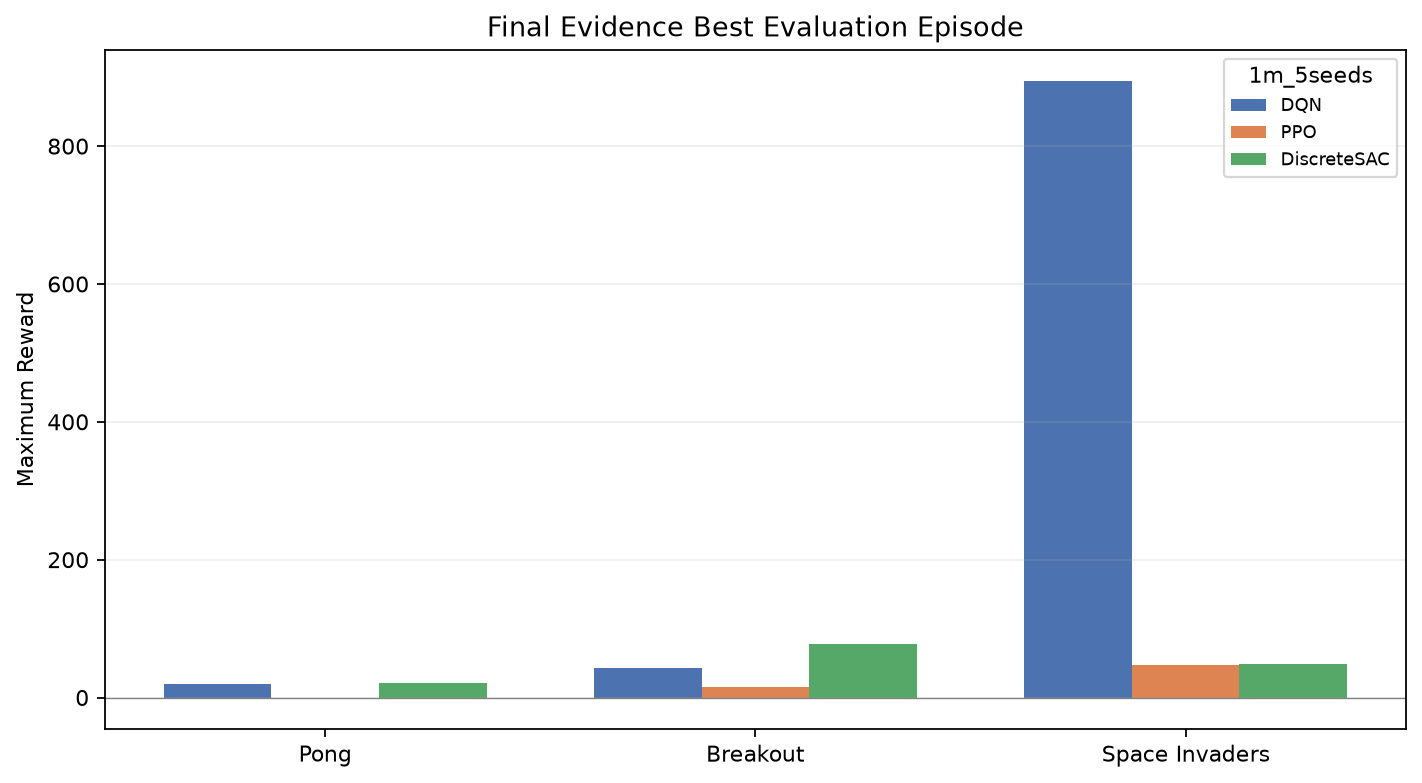
\includegraphics[width=0.95\linewidth]{max_reward.png}
\caption{Maximum reward. This plot shows the best episode score reached in evaluation. It helps identify policies that occasionally perform well even when their mean performance is unstable.}
\end{figure}

\begin{figure}[H]
\centering
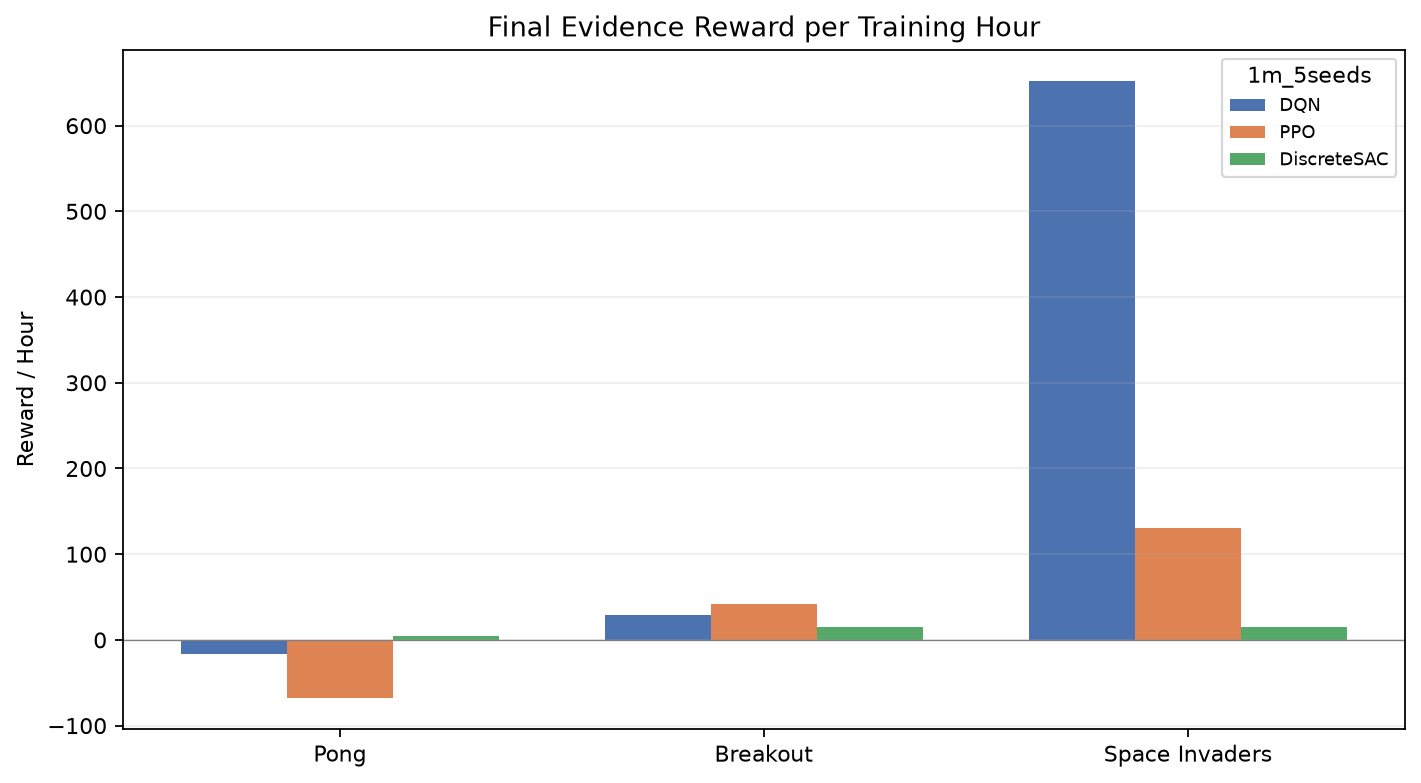
\includegraphics[width=0.95\linewidth]{reward_per_hour.png}
\caption{Reward per hour. This plot normalizes reward by training wall-clock time. It is useful because PPO, DQN, and custom DiscreteSAC have very different runtime costs.}
\end{figure}

\begin{figure}[H]
\centering
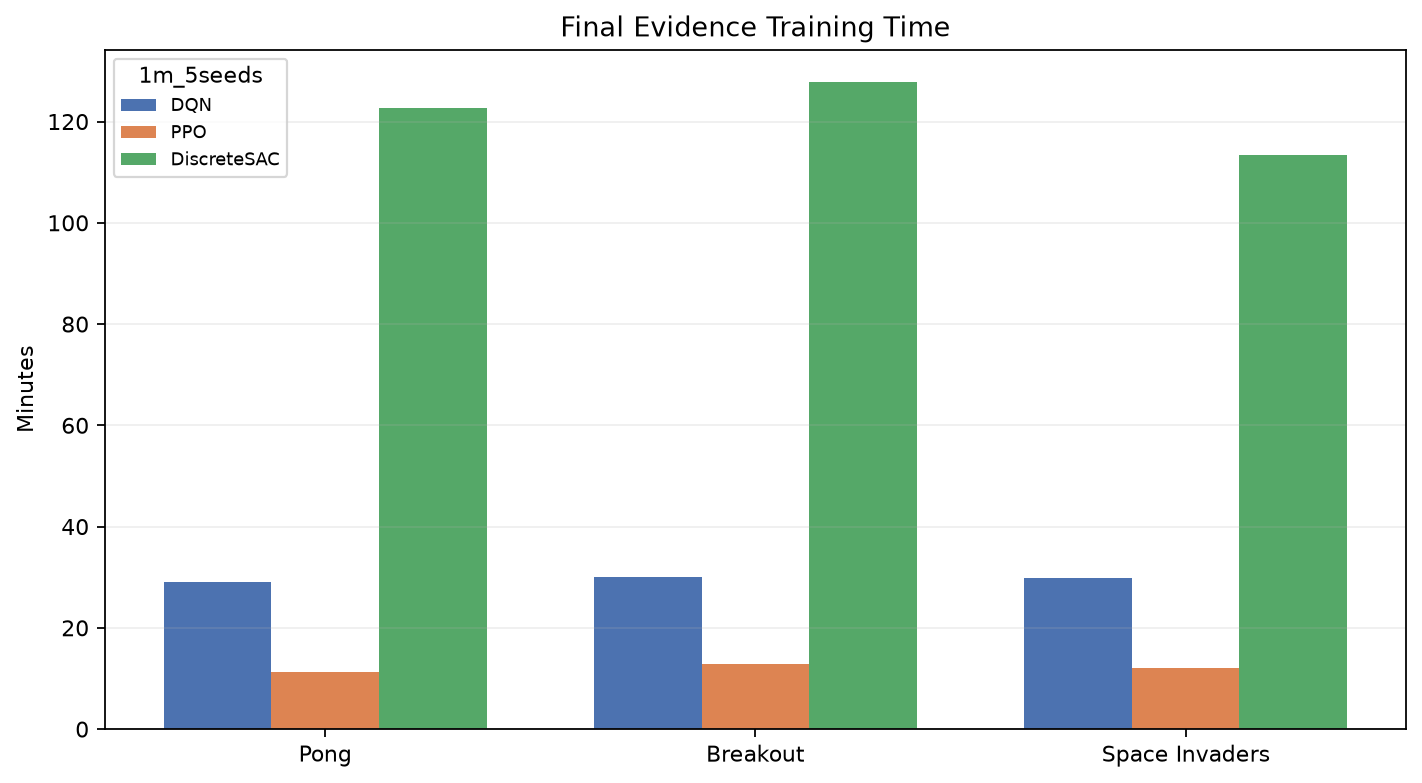
\includegraphics[width=0.95\linewidth]{training_time.png}
\caption{Training time. This plot compares wall-clock training time. It highlights the engineering cost of the custom DiscreteSAC loop relative to the Stable Baselines3 implementations.}
\end{figure}

\subsection*{DQN Final Results: \texttt{1m\_5seeds}}

DQN is the most stable final baseline. The \texttt{1m\_5seeds} profile contains five seeds for each game. Each seed was evaluated over 100 episodes.

\begin{longtable}{L{0.28\textwidth} r r r r}
\toprule
Game & Seeds & Mean of seed means & Seed std & Best episode max \\
\midrule
\endhead
Pong & 5 & -8.14 & 10.37 & 19 \\
Breakout & 5 & 14.66 & 3.68 & 43 \\
Space Invaders & 5 & 324.66 & 26.43 & 895 \\
\bottomrule
\end{longtable}

Interpretation: DQN remained the strongest Space Invaders baseline by a large margin and produced stable Breakout performance. Pong was seed-sensitive at the 1M-step budget: some seeds learned meaningful play while others stayed weak.

\subsection*{PPO Final Results: \texttt{1m\_5seeds}}

The final PPO evidence now comes from the same \texttt{1m\_5seeds} profile as DQN and DiscreteSAC. The earlier dedicated diagnostic profile remains useful for explaining the debugging process, but the final reported PPO numbers below are the completed five-seed benchmark values.

\begin{longtable}{L{0.28\textwidth} r r r r}
\toprule
Game & Seeds & Mean of seed means & Seed std & Best episode max \\
\midrule
\endhead
Pong & 5 & -12.81 & 4.55 & -1 \\
Breakout & 5 & 8.97 & 2.34 & 15 \\
Space Invaders & 5 & 26.20 & 4.57 & 47 \\
\bottomrule
\end{longtable}

Interpretation: PPO is the fastest final algorithm by wall-clock time, but its 1M-step performance remained weak. It underperformed DQN on all three games and underperformed DiscreteSAC on Pong and Breakout. This is consistent with the earlier diagnostic observation that PPO can require larger Atari budgets or closer reference hyperparameters before it becomes competitive.

\subsection*{DiscreteSAC Final Results: \texttt{1m\_5seeds}}

The final DiscreteSAC evidence now comes from the completed five-seed \texttt{1m\_5seeds} profile after the playback and training-recipe fixes discussed above.

\begin{longtable}{L{0.28\textwidth} r r r r}
\toprule
Game & Seeds & Mean of seed means & Seed std & Best episode max \\
\midrule
\endhead
Pong & 5 & 8.41 & 16.75 & 21 \\
Breakout & 5 & 32.47 & 3.66 & 77 \\
Space Invaders & 5 & 29.53 & 0.42 & 49 \\
\bottomrule
\end{longtable}

Interpretation: DiscreteSAC is the strongest final algorithm on Pong and Breakout by mean reward, but its Pong result has very high seed variance because one seed collapsed while several seeds performed well. It remained weak on Space Invaders, where DQN was clearly stronger. This supports the project conclusion that the custom Stable DiscreteSAC-style recipe improved the algorithm, but Space Invaders still needs better long-horizon credit assignment and/or a closer SD-SAC implementation.

\subsection*{Broader Benchmark Context}

Older pilot profiles are still useful for understanding the project development.

\begin{longtable}{L{0.22\textwidth} L{0.20\textwidth} r r r}
\toprule
Profile & Algorithm & Pong & Breakout & Space Invaders \\
\midrule
\endhead
\texttt{100k\_1seed} & DQN & -21.00 & 7.65 & 187.50 \\
\texttt{100k\_1seed} & PPO & -21.00 & 0.00 & 285.00 \\
\texttt{100k\_1seed} & DiscreteSAC & -21.00 & 0.00 & 168.25 \\
\texttt{200k\_1seed} & DQN & -21.00 & 8.25 & 170.00 \\
\texttt{200k\_1seed} & PPO & -21.00 & 2.70 & 285.00 \\
\texttt{200k\_1seed} & DiscreteSAC & -21.00 & 0.00 & 0.00 \\
\bottomrule
\end{longtable}

The short pilots showed that 100k-200k timesteps were not enough for reliable Pong behavior and that the earlier DiscreteSAC settings were fragile. These failures were useful because they led to the diagnostic profiles, action logging, playback generation, stochastic DiscreteSAC playback, and the newer stable recipe.

\subsection*{Qualitative Playback Findings}

Playback videos changed the interpretation of the numeric results. PPO and DiscreteSAC sometimes produced action distributions that looked acceptable in CSV form but poor in video. The most important qualitative observations were:

\begin{itemize}
\item Pong requires coherent ball tracking; random-looking paddle movement is not enough.
\item Breakout can look good until life loss; without post-life FIRE handling, full-game video can appear stuck.
\item Space Invaders can get nonzero score by shooting, but a good policy should also move, aim, and dodge.
\end{itemize}

This is why the final benchmark keeps both CSV metrics and MP4 playback videos.

\section*{5 - Conclusion}

This project produced a complete Atari RL benchmarking pipeline and a set of interpretable results across DQN, PPO, and DiscreteSAC. The final benchmark is now fair across the three algorithms because all final results use the same \texttt{1m\_5seeds} profile, the same three games, and the same five seeds. The project includes the core elements expected from a rigorous RL benchmark: defined observation/action/reward spaces, shared preprocessing, controlled configurations, checkpointing, result CSVs, manifests, diagnostics, logs, and playback videos.

DQN is the clearest final baseline on Space Invaders and remains the most dependable reference implementation. PPO was fastest wall-clock but weaker in reward at this 1M-step budget. DiscreteSAC required the most debugging because it is custom and less standardized for Atari; after the fixes, it became the strongest mean performer on Pong and Breakout, but it was slow and still weak on Space Invaders.

The main technical problems solved during the project were:

\begin{itemize}
\item separating profile outputs and preventing overlapping runs with locks;
\item adding algorithm filtering for focused diagnostics;
\item adding playback videos and playback metadata;
\item adding PPO and DiscreteSAC diagnostics;
\item keeping SAC discrete rather than incorrectly using continuous SAC;
\item fixing DiscreteSAC numerical and policy-collapse issues;
\item fixing Breakout full-game playback after life loss;
\item adding a one-line playback regeneration helper;
\item moving DiscreteSAC hyperparameters closer to reference Atari SAC practice.
\end{itemize}

The main lesson is that reward tables alone are not enough. A policy can score nonzero while behaving poorly, especially in Space Invaders. Playback and diagnostics are necessary to understand whether an agent is actually learning the intended behavior.

Recommended future work:

\begin{enumerate}
\item Increase PPO and DiscreteSAC budgets beyond 1M timesteps if time permits.
\item Add confidence intervals and formal seed-level statistical tests.
\item Add closer SD-SAC features such as n-step returns and stored entropy penalties.
\item Parse TensorBoard logs into learning curves for the final report figures.
\item Review the failed or weak playback seeds qualitatively, especially DiscreteSAC Pong seed 0 and all Space Invaders policies.
\end{enumerate}

References used for method direction:

\begin{enumerate}
\item Schulman, J., Wolski, F., Dhariwal, P., Radford, A., and Klimov, O. ``Proximal Policy Optimization Algorithms.'' arXiv:1707.06347, 2017. \url{https://arxiv.org/abs/1707.06347}
\item Haarnoja, T., Zhou, A., Abbeel, P., and Levine, S. ``Soft Actor-Critic: Off-Policy Maximum Entropy Deep Reinforcement Learning with a Stochastic Actor.'' Proceedings of ICML, 2018. \url{https://arxiv.org/abs/1801.01290}
\item Christodoulou, P. ``Soft Actor-Critic for Discrete Action Settings.'' arXiv:1910.07207, 2019. \url{https://arxiv.org/abs/1910.07207}
\item Stable Baselines3 Contributors. ``Stable Baselines3 Documentation: DQN and PPO.'' \url{https://stable-baselines3.readthedocs.io/}
\item Huang, S., Dossa, R. F. J., Raffin, A., Kanervisto, A., and Wang, W. ``CleanRL: High-quality single-file implementations of deep reinforcement learning algorithms.'' Journal of Machine Learning Research, 2022. \url{https://github.com/vwxyzjn/cleanrl}
\item Zhou, H., Lan, T., and Aggarwal, V. ``Revisiting Discrete Soft Actor-Critic.'' arXiv:2209.10081, 2022. \url{https://arxiv.org/abs/2209.10081}
\end{enumerate}

Project repository: \href{https://github.com/elsayedelmandoh/atari-rl-benchmarking}{elsayedelmandoh/atari-rl-benchmarking}

\end{document}
